% THIS IS SIGPROC-SP.TEX - VERSION 3.1
% WORKS WITH V3.2SP OF ACM_PROC_ARTICLE-SP.CLS
% APRIL 2009
%
% It is an example file showing how to use the 'acm_proc_article-sp.cls' V3.2SP
% LaTeX2e document class file for Conference Proceedings submissions.
% ----------------------------------------------------------------------------------------------------------------
% This .tex file (and associated .cls V3.2SP) *DOES NOT* produce:
%       1) The Permission Statement
%       2) The Conference (location) Info information
%       3) The Copyright Line with ACM data
%       4) Page numbering
% ---------------------------------------------------------------------------------------------------------------
% It is an example which *does* use the .bib file (from which the .bbl file
% is produced).
% REMEMBER HOWEVER: After having produced the .bbl file,
% and prior to final submission,
% you need to 'insert'  your .bbl file into your source .tex file so as to provide
% ONE 'self-contained' source file.
%
% Questions regarding SIGS should be sent to
% Adrienne Griscti ---> griscti@acm.org
%
% Questions/suggestions regarding the guidelines, .tex and .cls files, etc. to
% Gerald Murray ---> murray@hq.acm.org
%
% For tracking purposes - this is V3.1SP - APRIL 2009

\documentclass{edm_template}

\usepackage{booktabs}
\usepackage{subfig}
\usepackage{graphicx}

\begin{document}

\title{QuanTyler : Apportioning Credit for Student Forum Participation}
%\subtitle{[Extended Abstract]
%\titlenote{A full version of this paper is available as
%\textit{Author's Guide to Preparing ACM SIG Proceedings Using
%\LaTeX$2_\epsilon$\ and BibTeX} at
%\texttt{www.acm.org/eaddress.htm}}}
%
% You need the command \numberofauthors to handle the 'placement
% and alignment' of the authors beneath the title.
%
% For aesthetic reasons, we recommend 'three authors at a time'
% i.e. three 'name/affiliation blocks' be placed beneath the title.
%
% NOTE: You are NOT restricted in how many 'rows' of
% "name/affiliations" may appear. We just ask that you restrict
% the number of 'columns' to three.
%
% Because of the available 'opening page real-estate'
% we ask you to refrain from putting more than six authors
% (two rows with three columns) beneath the article title.
% More than six makes the first-page appear very cluttered indeed.
%
% Use the \alignauthor commands to handle the names
% and affiliations for an 'aesthetic maximum' of six authors.
% Add names, affiliations, addresses for
% the seventh etc. author(s) as the argument for the
% \additionalauthors command.
% These 'additional authors' will be output/set for you
% without further effort on your part as the last section in
% the body of your article BEFORE References or any Appendices.

\numberofauthors{3} %  in this sample file, there are a *total*
% of EIGHT authors. SIX appear on the 'first-page' (for formatting
% reasons) and the remaining two appear in the \additionalauthors section.
%
\author{
% You can go ahead and credit any number of authors here,
% e.g. one 'row of three' or two rows (consisting of one row of three
% and a second row of one, two or three).
%
% The command \alignauthor (no curly braces needed) should
% precede each author name, affiliation/snail-mail address and
% e-mail address. Additionally, tag each line of
% affiliation/address with \affaddr, and tag the
% e-mail address with \email.
%
% 1st. author
\alignauthor
Ankita Bihani\\
       \affaddr{Stanford University}\\
       \affaddr{Stanford, USA}\\
       \email{ankitab@stanford.edu}
% 2nd. author
\alignauthor
% 3rd. author
\alignauthor Andreas Paepcke\\
       \affaddr{Stanford University}\\
       \affaddr{Stanford, USA}\\
       \email{paepcke@cs.stanford.edu}
\and  % use '\and' if you need 'another row' of author names
% % 4th. author
% \alignauthor Lawrence P. Leipuner\\
%        \affaddr{Brookhaven Laboratories}\\
%        \affaddr{Brookhaven National Lab}\\
%        \affaddr{P.O. Box 5000}\\
%        \email{lleipuner@researchlabs.org}
% % 5th. author
% \alignauthor Sean Fogarty\\
%        \affaddr{NASA Ames Research Center}\\
%        \affaddr{Moffett Field}\\
%        \affaddr{California 94035}\\
%        \email{fogartys@amesres.org}
% % 6th. author
% \alignauthor Charles Palmer\\
%        \affaddr{Palmer Research Laboratories}\\
%        \affaddr{8600 Datapoint Drive}\\
%        \affaddr{San Antonio, Texas 78229}\\
%        \email{cpalmer@prl.com}
}
% There's nothing stopping you putting the seventh, eighth, etc.
% author on the opening page (as the 'third row') but we ask,
% for aesthetic reasons that you place these 'additional authors'
% in the \additional authors block, viz.
% \additionalauthors{Additional authors: John Smith (The Th{\o}rv{\"a}ld Group,
% email: {\texttt{jsmith@affiliation.org}}) and Julius P.~Kumquat
% (The Kumquat Consortium, email: {\texttt{jpkumquat@consortium.net}}).}
% \date{30 July 1999}
% Just remember to make sure that the TOTAL number of authors
% is the number that will appear on the first page PLUS the
% number that will appear in the \additionalauthors section.

\maketitle
\begin{abstract}
%  We develop a random forest classifier that helps assign academic
%  credit for a student's class forum participation. Our twelve predictors
%  are quantities that are easily available from typical forum facilities, such
%  as number of endorsed contributions, number of questions asked, number of answers, and number of posts viewed. We add page rank and centrality to these base measures. The classification target are the four classes created by
%  student rank quartiles. Course content experts provided ground truth
%  by ranking a limited number of post pairs. We expand this labeled set
%  via data augmentation. We compute the relative importance of the
%  predictors, and compare performance in matching the human expert
%  rankings, as we vary the number of predictors used in training. We
%  reach multiclass AUC measures between 0.64 and 0.94, depending on the
%  number of deployed predictors. This performance is compared with the
%  simple formulae that are currently used by some instructors for
%  estimating the amount of credit to apportion for forum activity in
%  their classes. To test generality and scalability,  we trained the
%  classifier on the archive of the Economics Stack Exchange
%  reputation data. We used this classifier to predict the quartile
%  assignments by human judges of forum posts from a University Artificial Intelligence course. Our first attempt at transfer learning reaches an average
%  AUC of 0.69.

We develop a random forest classifier that helps assign academic
credit for a student's class forum participation. The classification
target are the four classes created by student rank quartiles. Course
content experts provided ground truth by ranking a limited number of
post pairs. We expand this labeled set via data augmentation. We
compute the relative importance of the predictors, and compare
performance in matching the human expert rankings. We reach an
accuracy of 0.96 for this task.  To test generality and scalability,
we trained the classifier on the archive of the Economics Stack
Exchange reputation data. We used this classifier to predict the
quartile assignments by human judges of forum posts from a university
Artificial Intelligence course. Our first attempt at transfer learning
reaches an average AUC of 0.66 on the augmented test set.

\end{abstract}

%% A category with the (minimum) three required fields
%\category{H.4}{Information Systems Applications}{Miscellaneous}
%%A category including the fourth, optional field follows...
%\category{D.2.8}{Software Engineering}{Metrics}[complexity measures, performance measures]
%
%\terms{Theory}
\keywords{Online Discussion Forum, MOOCs, residential courses, random forest, credit computation, online learning, transfer learning, instructor support, collaborative learning, grading, crowdsourcing, forum assessment.} % NOT required for Proceedings

% Points to make:
%    - Forums are used no matter what the lit says.
%    - We begin with all available predictors, and show which ones are
%      important. 
%    - Generalizability: Econ stackexchange.
%    - No cheating detection yet; though add the near-dups
%    - Measures --> Predictors.
%    - Conclusion: spam: some predictors spamable, others harder.
%    - Piazza screenshot.

\section{Introduction}
Massively Open Online Courses (MOOCs) have in past years provided
content to populations outside traditional venues of higher
education. For these settings, online forum facilities that are
built into the course delivery platforms, such as Coursera and Open
edX are the primary means of communication among learning peers, and
for interacting with instructors.

Beyond the practical needs for coordinating logistics in
geographically distributed settings, online discussion forums can serve pedagogical
goals as well. 
% The process of discussions is a critical dimension of the learning process. 
Online asynchronous discussion forums provide the basis for collaborative learning, which enhances critical thinking \cite{gokhale1995collaborative}. Students answering each others' questions can be
helpful for all parties \cite{supers}. This support function is
particularly useful in Science and Engineering courses. But as
discussion centric humanities courses embrace distance learning, discussions
on online forums will likely gain even more prominence.

However, it is not only in the context of distance learning that forum
facilities have found uses. Even when in person class time is
available, many residential college courses have adopted the tool. The
need for students to ask questions, voice concerns, or to point out
errors in course material are as salient in residential settings as
they are in less traditional situations, such as distance learning \cite{andresen2009asynchronous}. 
% TODO Please read this part(start)
Figure~\ref{fig:forumGrowth} shows the rapid growth in the volume of contributions per year to
Piazza, just one of the several available online forum tools in a large private university. Despite the fact that the total number of Piazza participants were roughly the same from 2012 to 2017 (with a slight peak in 2013), the total volume of contributions increased monotonically. It is possible that this rapid increase in the volume of contributions per year on Piazza stems from the increasing popularity and growing adoption of the Piazza forum among students and instructors for collaborative discussions. 
% TODO: Please read this part(end)
\begin{figure}
\centering
  \includegraphics[width=1.0\columnwidth]{Figs/growth2}
  \caption{Number of Piazza forum contributions and participants per year for courses at our University }~\label{fig:forumGrowth}
\end{figure}

Given the importance of collaborative discussion in the learning
process at both the theoretical and empirical level, instructors in at
least some universities are assigning between 1\% and 25\% of their course grading component to online forum contribution. % Despite office hours held by numerous course assistants, students helping each other online is helpful. Not
% only does student activity make more answers available for future use, but responses are provided very quickly in many cases, as students in residential
% settings follow similar working hours.
Two primary challenges arise when apportioning course credit to reward students' forum contribution. First, students can attempt to game the system. On surveying some instructors, we learnt about instances of students copying a peer's forum posts, adding spaces or
other innocuous characters to fool automated contribution counters. Thus, the system needs to be able to flag such instances.

A second, more complicated problem is that of apportioning fair credit
to the students at the end of the quarter. Forum contributions take many
forms. Asking an insightful or intriguing question can contribute as
much to the course as providing answers. Taking the time to view
other students' contributions is a contribution as well. However, for courses
with hundreds of students, manual assessment of every forum post by
each student in order to assign a forum participation score is not
feasible. On surveying some instructors, we learnt that they instead develop ad--hoc formulae over the participation
statistics provided by the forums, hoping to capture the right signals. This
practice can not only lead to non-uniform grading (based on
diverging intuitions) across courses, but also fail in rewarding students with a fair forum participation credit commensurate with their effort.

In addition to the above two challenges, there is untapped potential
from today's use of forum facilities. As courses are offered
repeatedly over the years, a treasure of course knowledge accumulates
in forum archives. The detection of high value forum contributions can
inform content selection from such archives.

In an effort to address these problems we are developing a coherent
system for boosting the value of online discussion
forums. Figure~\ref{fig:arch} shows a block diagram of our proposed
system.
\begin{figure}
\centering
\includegraphics[width=0.6\columnwidth]{Figs/systemBlockDiagram.png}
  \caption{Block diagram of our proposed framework around forum facilities.}
  ~\label{fig:arch}
\end{figure}
In this paper, we focus on {\em QuanTyler}, the module responsible for helping with automatic forum credit
apportioning. This component is highlighted in the figure. We plan to make the operation of $QuanTyler$ customizable by instructors. For instance, instructors will
be able to decide the granularity of partitioning the class into their
quantiles of choice. 
% We briefly cover the Spam detector component as well, in this paper.

We begin with describing how we used human judgments to establish ground truth of what a
`good' and credit-worthy forum contribution looks like. This ground truth is used for measuring success, and for training the models. At the heart of our contribution are three experiments whose outcomes
are required to inform the development of the $QuanTyler$ module. These experiments are outlined below.

In the first experiment, we explore how students can be classified
into quantiles based on their forum contributions, such that the
implied ranking matches the ground truth. We show the hyperparameters
needed to make a Random Forest classifier work well in support of the
post evaluation task. We reached a high $AUC$ measure in this task.

However, obtaining human judgments is expensive. At the same time,
this requirement for human judgment would limit the ability to create
classifiers for many courses. To break out of this confinement, we
examine how a much larger source of labels for a forum-like enterprise
might be used for training, and to test generalizability.

To this purpose we used \emph{Stack Exchange}, \cite{stackex} which is an online Q \& A platform with millions of users. Stack Exchange is partitioned into sites for varying disciplines. We
chose the Economics archive \cite{stackexEcon}, and used it as a source for
attempting transfer learning. In our second experiment we trained a
random forest model on Stack Exchange reputation data, and tried
predicting the quality ratings of human expert-rated forum posts in an Artificial
Intelligence (AI) class. While not as good a classifier as the one
trained on the forum data itself, this first attempt at transfer
learning reached an $AUC = 0.69$, which we hope to improve further going
forward. However, the data from Stack Exchange cannot be used in
its raw form to build a classifier, and we will cover the required
processing in Section~\ref{sec:exp2}.

In our third experiment, we demonstrated that (at least one
of) the ad--hoc formulas currently deployed at our university diverges significantly from human experts' judgment.

\section{Related work}

Online discussion forums empower students and instructors to engage
one another in ways that promote critical thinking, collaborative
problem solving, and knowledge construction
\cite{pendry2015individual, marra2004content}. Research has
shown that linking some form of assessment to forum participation is an
important element in promoting and enhancing online
interactivity \cite{laurillard2013rethinking, yeh2005use}. 


Quantitative methods for content analysis are most widely used in
assessing effective forum participation. \cite{de2006content} presents
an overview of 15 different content analysis instruments used in 
computer supported collaborative learning (CSCL) studies.

The model proposed by \cite{henri1992computer} is a common starting
point in many CSCL studies. In \cite{henri1992computer}, the author presented a framework and analytical model to evaluate computer-mediated communication (CMC). The analytical model was developed to highlight five key dimensions of the learning process exteriorized in messages: 
{\em participation, interaction, social, cognitive and metacognitive dimensions}. Although this model provides an initial framework for coding CMC discussions, it lacks detailed criteria for systematic and robust classification of electronic discourse \cite{howell1996methodology}.


Many researchers have strongly endorsed Social Network Analysis as a
key technique in assessing the effectiveness of forum interactions
\cite{de2007investigating, yusof2009students,
  dowell2015modeling}. Social Network Analysis is a research
methodology that seeks to identify underlying patterns of social
relations based on the way actors are connected with each other
\cite{wasserman1994social, scott2011sage}.

 
In \cite{nandi2009conceptual}, the authors discuss a conceptual
framework for assessing quality in online discussion forums. Drawing
on previous work \cite{henri1992computer, newman1995content, garrison2001critical}, the authors propose three broad categories of criteria for assessing forum participation:{ \em content}, which demonstrates the type of skill shown by the learners,  {\em interaction quality}, which looks at the way learners interact with each other in a constructive manner, and {\em objective measures}, which highlight the frequency or participation. These three broad criteria are further divided, resulting in a total of 11 criteria. In order to support educators, the framework outlines a further sub classification, clearly indicating what may be a poor, satisfactory, good or excellent performance against each criterion. The primary limitation of this study is that manual assessment by instructors is not feasible in courses with hundreds of students.

In \cite{wang2015investigating}, the authors adopt a content analysis approach and develop a coding scheme to analyze students' discussion behaviors in order to categorize them as active, constructive or interactive. However, the authors do not discuss how to apportion forum participation credit based on the behaviors depicted. One of their findings shows that higher quantity of participation in the MOOC discussion forums is associated with higher learning gains. In coherence with this finding, we also include participation count as one of our potential predictors. 


To the best of our knowledge, the most closely related work to our paper are \cite{rabbany2014collaborative} and \cite{shaul2009assessing}.

In \cite{rabbany2014collaborative}, the authors present the use of Social Network Analysis (SNA) to examine the structure and composition of ties in a given network, and provide insights into its structural characteristics. In particular, the authors rely on two types of networks: interaction network between students in a course, and the network of terms used in their interactions. The dynamic visualization of interaction between participants and the groups or communities formed can help the instructors rank students based on their centrality in the students' interaction network. Visualizing the network of terms used in an online discussion forum can be used to compare the interest of different students and their relative engagement. 


In \cite{shaul2009assessing}, the author proposes the use of the
following metrics to assess forum participation: initiative,
effectiveness--depth, effectiveness--breadth, value, timeliness,
participation, scholarship, style, and instructor points. Our system explicitly or implicitly covers most of these measures and augments them further by adding the crucial element of social network analysis to assess forum participation.

In contrast with both the aforementioned contributions, each of which
focuses on specific aspects for assessing forum participation, our
approach for assessing a student's contribution uses a combination of
quality measures, quantitative measures, engagement level measures and
also measures from social network analysis. The intent is to provide a holistic view of each student's contribution. We develop a system that the instructors can customize and easily use for apportioning forum participation credit.


\section{Current Practice}

Many universities use the Piazza forum facility \cite{Piazza} for asynchronous online discussions. In order to provide context for the experiments below, we provide a brief overview of this tool.

Piazza is a Q\&A web service for online discussions, where users can
ask questions, answer questions, and post notes. The user interface contains a dynamic list of
posts, which are question titles followed by a snippet of lines from
the post. 
% The posts are arranged chronologically on the left panel,
% while the central panel is meant for viewing posts and adding
% contributions. 
For every question, there is a placeholder for the
instructor's answer, which can only be edited by
instructors. There is also a students' answer section where students
{\em collaborate} to construct a single answer. Students can {\em upvote} each others' questions or answers. Instructors can also {\em endorse} good questions and answers, which are then highlighted as instructor endorsed. There is also a discussion segment for follow-up threads.
Figure~\ref{fig:piazza} shows a snapshot of the Piazza discussion forum.

\begin{figure}
\centering
\includegraphics[width=1.0\columnwidth]{Figs/Piazza4.png}
  \caption{Sample annotated screenshot of the Piazza forum facility.}
  ~\label{fig:piazza}
\end{figure}


% Piazza provides the instructors with certain statistics for each
% student. These statistics are: number of questions asked, number of
% questions answered, total number of contributions (including posts,
% responses, edits, follow-ups etc.), the number of days the student was online, and the total number of posts viewed by the student. 

On surveying several instructors who consider Piazza forum participation in their
grading scheme, we found that most rely on
the basic quantitative statistics that the forum machinery readily
offers. The following were some of the grading schemes that are
currently used by instructors at our university for awarding forum
participation grades:\\ \\ 
% \begin{itemize}
\emph{Scheme~1}: In this scheme, scores of each student were calculated using the following formula:
\begin{equation}
\begin{split}
\texttt{Score} = 1 * \texttt{(no\_questions\_asked)} + 
\\ 4 * \texttt{(no\_questions\_answered)} + \\
0.5* \texttt{(other\_contributions)}
\end{split}
\end{equation}
\emph{Scheme~2}: In this scheme, scores of each student were calculated using the following formula:
\begin{equation}
\begin{split}
\texttt{Score} = 3 * \texttt{(no\_questions\_answered)} + \\ 
1* \texttt{(no\_followups)}
\end{split}
\end{equation}

Anyone above the 90\textsuperscript{th} percentile received full
credit, and all the other students received a score of
0.\\ 
\emph{Scheme~3}: Award full credit if at least one forum contribution
was made, and the student was online on the forum for at least $x$
number of days, or viewed at least $y$ posts. Here $x$ and $y$ were
set by the instructor using intuition. \\ \emph{Scheme~4}: Award full
credit to a student if they made at least one contribution to the
forum. 


% \end{itemize}


All the above methods rely solely on the basic statistics directly
provided by Piazza \cite{Piazza}. The concern, however, is whether these methods
accurately and meaningfully award credit to the deserving
students. Following are two major limitations of using the current
grading schemes: \squishlist
\item \emph{Lack of quality measures :} All the 4 grading schemes described above
  overlook the quality of contributions. This exclusion negatively
  impacts the grades of the students who post few, but very high quality
  contributions. More importantly, relying
  solely on the quantity of the contributions encourages posts that 
  do not constitute meaningful forum participation. This behavior, in turn, can cause the forum's
  quality to devolve.
\item \emph{Reward not proportionate to effort :} Most of these
  schemes fail to award credit proportionate to the amount of effort
  and time the student invested. For instance, using the third or
  fourth scheme means that two students with vastly varying quantity
  and quality of contributions would be awarded the same score.
  Concretely, let us consider two students $A$ and $B$. Student $A$
  made only one forum contribution during the course by posting a ``+1"
  to another student's question. However, student $B$ regularly made
  meaningful forum contributions throughout the quarter. Using grading
  scheme 4, both would receive equal credit. This lack of fairness can deter students from engaging in meaningful forum contributions.
  \squishend

Despite the above limitations, instructors have no choice but to
rely on grading schemes like the ones discussed above. The large
volumes of forum posts that accumulate by the end of the term make it
impossible for the course staff to manually go through them to
apportion credit. However, even if hypothetically, one were to have
the course staff manually go through each of the contributions, there
is a significant amount of subjectivity in assessing forum
contributions. Having TAs manually grade contributions would lead to a
lack of grading uniformity. A trivial contribution according to one
TA, might be a significant contribution to another. Thus, there is a
need for an automated way to assess the forum participation of
students using a holistic grading scheme. Automation can lead to a
standardized approach across the entire class.

The next sections discuss how we developed a system to assess forum
participation by each student at scale. We go beyond the ready at hand
statistics that are provided by the forum, and additionally
incorporate measures that provide insight into the dynamics of
students interacting in the forum. These dynamics manifest in the
social networks that are created by the online interactions. We
briefly review candidate predictors in the next section.

\section{Potential Predictors}

The measurements of predictors arise from the data sets generated by
forum facilities during the length of an academic term. Each offering of
a course generates a separate data set, such as the one we used from
the AI course.

\textbf{Quantitative measures}: These measures reward based on the volume of contributions made by an individual. 
% Hypothetically, if all
% the contributions are assumed to be of identical quality, the time and
% effort invested by a student is directly proportional to the volume of
% contributions made by him/ her. Hence, the forum participation score
% should be directly proportional to the number of forum contributions
% made by the student. 
As discussed in \cite{wang2015investigating}, higher forum participation count translates to higher learning gains, hence we include quantitative features in our list of potential predictors. 
These four predictors are: \emph{number of questions
  asked}, \emph{number of questions answered}, \emph{total number of
  contributions}, and \emph{average post length} by a student.

% 	\begin{itemize}
%     \item Number of questions asked
%     \item Number of questions answered
%     \item Total number of contributions
% 	\end{itemize}
    
\textbf{Engagement level measures}: In order to reward the students
who started important or intriguing threads, which in turn engaged
many students, the \emph{average number of collaborators} in the
threads started by the student was added as a predictor. A second
predictor, \emph{average number of views} received by a student's questions was added for similar reasons. Given that not everyone in the
class might be comfortable actively posting on the forum, we use some metrics to reward the passive engagement of the students. Some of the
students are great listeners; they view or follow most of the posts,
and are regularly online on the forum, which translates to passive forum participation. The two predictors we used to
apportion credit for passive collaboration on the forum are:
\emph{total number of days a student was logged into the forum}, and the number of \emph{posts viewed} by the student. 
  
%  The forum facility
% used by the class allows students to collectively work on the answer
% to a question. Participation in such work is recorded in the forum
% data set, and thus available as a candidate predictor.
% 	\begin{itemize}
%     \item Number of days a student was online on the forum
%     \item Number of posts viewed
% 	\end{itemize}
    
\textbf{Quality measures}: These measures are used to reward the
students based on the quality of their contributions. These include upvotes and endorsement counts available in forum
datasets. Students can express appreciation for a post by adding an
upvote to the contribution. Instructors can explicitly endorse answers
provided by students, marking those answers as definitive. Upvotes and
endorsements articulate human judgments, and can be thought of as
crowdsourcing post quality assessment.

Another strength of quality measures is their robustness to
student cheating by flooding the forum with meaningless threads to
increase their contribution count.  Our two quality predictors are:
\emph{number of endorsed answers by the student}, and
\emph{total number of endorsements}, including upvotes on the questions,
answers and instructors' endorsements.

% 	\begin{itemize}
%     \item Number of endorsed answers
% 	\item Total number of endorsements (including upvotes on the questions, answers and instructors' endorsements)
%     \end{itemize}

\textbf{Social Network Analysis}: As discussed in the Related work section, Social Network Analysis (SNA) provides insights to the student forum participation.  A brief detour in the following section provides
background for the measures we used for SNA.

In order to include
the SNA component in our credit apportioning
system, the following networks were extracted from the class forum
dataset. In the definitions below, nodes represent students and instructors. Typed edges
represent interactions that are possible in the forum. Link weights
encode the number of such interactions between the link's nodes.

\emph{Upvotes network}: An upvotes network is extracted, where an edge
from student $A$ to student $B$ indicates that $A$ upvoted $B$'s content at
least once, and the weight of the edge encodes the number of times $A$
upvoted $B$'s content.

\emph{Endorsement network}: An endorsement network is extracted, where
an edge from instructor $A$ to student $B$ indicates that $A$ endorsed
$B$'s content at least once, and the weight of the edge encodes the
number of times $A$ endorsed $B$'s content.

\emph{Combined upvotes and endorsement network}: This construct is a union of
the above two networks. An edge from $A$ to $B$ indicates that $A$
either upvoted and/or endorsed $B$'s content at least once, and the
weight of the edge encodes the sum of the upvotes and endorsements.

\emph{Interaction network}: This graph models the interaction that
happened on the forum over the duration of the course. In the
interaction network, an edge from $A$ to $B$ indicates that $B$
responded at least once to a question that $A$ posted.
% \end{itemize}

We use these networks to derive our final two predictors: \emph{degree
  centrality} in the interaction network, and \emph{page rank} in the combined upvotes and endorsement network.

We calculate the degree centrality for every node in the interaction
network. Degree centrality measures the number of links incident upon
a node. Higher degree centrality of a student implies that the student
answered questions or resolved doubts for a large number of
students. On a high level, degree centrality in the interaction
network translates to the ``helpfulness" and ``resourcefulness" of the student. It also captures the breadth of the student's course knowledge.

Page rank in the combined upvotes and endorsement network was used in
order to capture importance in both upvotes and endorsement
information using a single metric. Page rank can additionally help
uncover influential or important students in the network. Their reach
extends beyond their immediate neighbors, and is therefore not
captured by the earlier described upvote/endorsement measures. The
higher the page rank in the combined network, the more ``influential" the
student.

\section{Ground Truth Collection}

In order to evaluate how effective each of the above predictors is in
informing credit apportioning, we obtained human judgments by paying former students and teaching
assistants of the AI or a related class to render judgments over a
sample of posts. Given the high course enrollment of 700+, not all the
posts could be evaluated. A survey instrument was used to collect the
judgments, and participants were paid a \$20 gift card. The number of
posts sampled was limited by this cost, and time capacity of the 24
participants we could recruit.

Each item in the survey for the experts was a pair of two posts by
different students. The experts were asked to indicate which of the
two contributions was more helpful for the class as a whole. (See the
precise instructions below). We chose this pairwise comparison method
to economize on raters' time and attention, and because the derivation
of full rankings from pairwise comparisons is well studied
\cite{heck2018,jami2011}.

The task in preparing the survey was to find forum contribution pairs
that would later help train an algorithm. The challenge was to select
a set of posts that would cover a range of measures for all our
candidate predictors, while being representative of the overall
contributions.  We describe here how this selection was accomplished.

Four algorithms use a weighted combination of the
above explained candidate predictors.

\squishlist
\item Alg~1: Using only quality measures and social network analysis measures.
\item Alg~2: Using only quantitative measures and engagement level measures.
\item Alg~3: Using all the measures with more emphasis placed on quantitative measures.
\item Alg~4: Using all the measures with more emphasis placed on quality measures.
\squishend
In addition, the current formula based grading scheme~1 that is used
by some instructors at our university is included as a variant. Let us call this approach Alg~5:
\begin{equation}
\begin{split}
\texttt{Score} = 1 * \texttt{(no\_questions\_asked)} + 
\\ 4 * \texttt{(no\_questions\_answered)} + \\
0.5* \texttt{(other\_contributions)}
\end{split}
\end{equation}

All the above five algorithms are then separately used to
calculate each student's score. 
Table~\ref{tab:kendall} shows the Kendall tau distance between the
rankings created by each of the algorithms. Most of the values in the
table are low, indicating low correlation between the rankings
calculated by each of the 5 algorithms. This result is intuitive because all the 5 algorithms were designed by us to capture slightly different signals.
As a next step, 10 new values are calculated,
each of which are absolute values of ranking differences between one
pair of rankings for the same student. Each algorithm pair is
processed. Thus, we have Alg1vsAlg2, Alg1vsAlg3, Alg1vsAlg4,
Alg1vsAlg5 and so on. For instance, if Student ID\# 500 was ranked 30
by Alg~1, and 300 by Alg~3, then the Alg1vsAlg3 value for Student ID\#
500 would be 270.

\begin{table}
  \centering
  \caption{Kendall tau distance between rankings created by the 5 algorithms}
  \label{tab:kendall}
  \begin{tabular}{@{}llllll@{}}
    \toprule
    & Algo1  & Algo2  & Algo3  & Algo4  & Algo5 \\ \midrule
    Algo1 & 1 & 0.8538   & 0.2213   & 0.7243   & 0.2268        \\
    Algo2 & 0.8538   & 1 & 0.2132   & 0.6621   & 0.2050        \\
    Algo3 & 0.2213   & 0.2132   & 1 & 0.2306   & 0.3064        \\
    Algo4 & 0.7243   & 0.6621  & 0.2306   & 1 & 0.2741   \\
    Algo5 & 0.2268  & 0.2050  & 0.3064   & 0.2741 & 1 
    \\ \bottomrule
  \end{tabular}
\end{table}


We then sort these ten rank differences in descending order. The top
entry in the 10 columns gives us the corner cases, or students `of interest'. To sample
student pairs, we compare these students of interest with the
students immediately above and immediately below in the ranking by
both the algorithm rankings under consideration. We clarify the procedure
with the following example:
% \begin{itemize}
\\Let us assume that student ID \#10 had the maximum absolute
difference between ranking through Alg~1 and Alg~3.  Also, using
Alg~1, student ID \#400 is directly above student ID \#10 and student
ID \#5 is directly below student ID \#10 in the ranking.  Finally, let
us assume that using Alg~3, student ID \#20 is directly above student
ID \#10 and student ID \#557 is directly below student ID \#10 in the
ranking.  Then posts by the student ID pairs of interest for which
human judgment was solicited
are: (10, 400), (10, 5), (10, 20), (10, 557).
% \end{itemize}
\\\\In addition to 40 such pairs of interest, additional student pairs were randomly sampled. At
most 4 question pairs and 4 answer pairs were sampled from all these
selected student pairs and presented to the experts. A total of 89
question pairs and answer pairs were used. In order to avoid fatiguing
the experts, the set was partitioned into two batches such that each
question pair or answer pair was voted on by at least 12 experts. The
set of judged samples thus served to inform boundary cases among
available measures, rather than to include every type of post. For
example, there was no attempt to cover all linguistic variations. The
addition of randomly sampled posts served to reach beyond this focus.

The survey instructions were as follows: \\ \emph{ Each of the
  following sections presents one pair of questions or answers that
  were posted to the course forum in the past. We ask that you to
  indicate for each pair, the contribution that might have been most
  helpful to the rest of the class.  }

One sample item from the survey is as follows:

\emph{
Q1: I am very confused about alpha-beta pruning, as we do not have example code from lecture. When we say we prune certain leaf, what does it mean? Does it mean we do not store that choices? \\
Q2: To create our own label, must it been binary label \{1,-1\} or it can be multi-categories with labels of any number? Is the feature still word counts or can be anything?\\
Which of the above two questions contributes more to the class community?
}

Note that in all cases the experts who answered the surveys were
different from the experts whose endorsements we counted when building
the classifier. 

% New section starts here 
In order to learn the experts' {\em intuition} about which of the predictors might
be important in ranking students' forum contributions, the following
related question was introduced in the ranking survey once at a random time,
with a facility to drag the entries up and
down to arrange the predictors in decreasing order of relevance:

\emph{Imagine you had the following statistics about forum
  contributions by all students at the end of the term. In your
  opinion, which statistics are important to evaluate the forum
  contributions of students to the class. Please drag the entries up
  and down to indicate their relative importance. The first entry
  would be the most important.  \squishlist
\item Number of questions asked by the student
\item Number of questions answered by the student
\item Total number of posts viewed by the student
\item Total number of days the student was online on the forum
\item Total number of endorsements received by the student
\item Total number of Forum contributions by the student (including
  questions, answers, notes, follow-ups, etc.)
\squishend
}

Based on the majority vote for every rank, we arrive at a ranking
order using the experts' intuition. This ranking was not used in any
of the experiments below. The information just illustrates the `gut'
feeling by our raters. The results are summarized in
Table~\ref{tab:faqRes}. Rank 1 is the most important feature. The
percentage of experts agreeing with each ranking is also included.

\begin{table}
\centering
\caption{Experts' intuitions for relative ordering of indicator
  importance. Example: 57.1\% of experts felt that the number of
  questions answered was the second-most important indicator.}
\label{tab:faqRes}
\begin{tabular}{lllc}
\hline
\centering \textbf{Rank} & \textbf{Feature} & \textbf{ \%support}  & \\ \hline
1 & \# of endorsements & 60.7   \\
2 & \# of questions answered & 57.1\\
3 & \# of Forum contributions & 46.4\\
4 & \# of questions asked & 46.4 \\
5 & \# of posts viewed & 60.7 \\
6 & \# of days online & 64.2    \\ \hline
\end{tabular}
\end{table}

% We compare these intuitions with our computationally determined
% predictor importance, in a later section.

\section{Experiment Preparation}
Given the pairwise rankings of posts by the experts we needed to
arrive at a ranking against which we could then train and test. We
generated this ranking using the Copeland method \cite{cope51}. The
procedure counts the number of times a student's post was considered
superior to the alternative post offered to an expert. The number of
losses are then subtracted from these wins. Copeland ranking ties can be broken by a \emph{second order Copeland} approach \cite{ties}. However, we found that forcing a complete order did not lead to good classification, because the ties are a reflection of true similarity.

We included at most 4 question pairs and 4 answer pairs from each sampled student in the survey. However, in most cases the sampled students had less than 4 questions / 4 answers. The final result was a list of 37 students for which we had
rankings from twelve experts each. We collected this large number of
rankings for each student because of the above mentioned subjectivity
in evaluating posts. In addition to the rankings, we also had the
measures for all our 12 candidate predictors for each of the 37
students .

%% Figure~\ref{fig:predDist} shows the distribution of the
%% measures after centering and scaling.

%% \begin{figure}[H] 
%% % \label{fig:rankGrpHist}  
%% \centering
%%   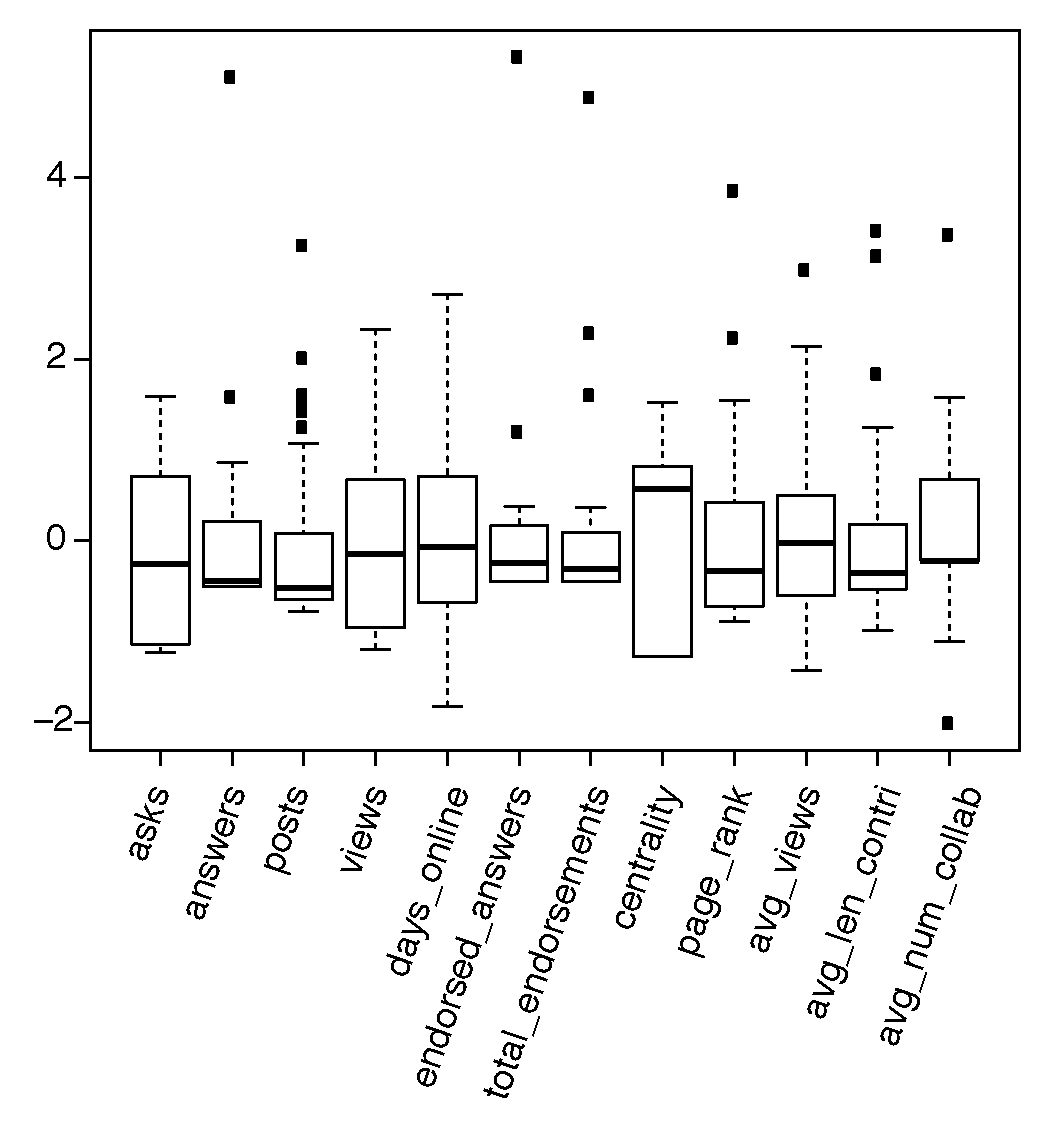
\includegraphics[width=0.8\columnwidth]{Figs/forum_predictor_box_plot1.pdf}
%%   \caption{Distribution of predictor measures from 37 students.}
%%   ~\label{fig:predDist}
%% \end{figure}

%% We examined the outliers and found that they are legitimate data
%% points. This finding supports \cite{supers}, which detected `super
%% posters' in MOOC forum activities.

Rather than attempting a regression, we formulated the problem as one
of classification into four classes: the rank quartiles. This decision
was based on the application of apportioning credit. A granularity of
four suffices, given that forum participation is not the only source
of credit for a course. Partitioning a ~5\% course credit into 700
values is not meaningful. 

Given the sparsity of our human labeled set, we first augmented the
labeled data as follows. We partitioned the ranked list of students
into four roughly equal parts. Figure~\ref{fig:augment}{\em a} shows the
top two partitions using fictitious numbers for clarity.
\begin{figure}[H] 
\centering
  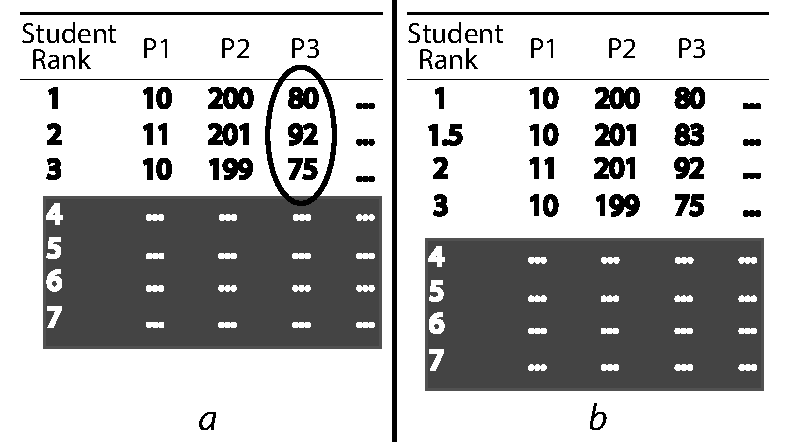
\includegraphics[width=0.8\columnwidth]{Figs/augmentation.pdf}
  \caption{Augmentation occurs separately within each quantile. Each column
    holds the measures of one predictor $P_n$. The top two quantiles
    are shown. Part~a: before augmenting the top quantile; Part~b:
    after augmentation.}  ~\label{fig:augment}
\end{figure}
\vspace{-2.5cm}
We then determined the range of values for each predictor within one
quartile. Finally, we generated new rows within each quartile by
randomly choosing values for each of its predictors from within the
range of values that the predictor took on within that quartile.

The four quantiles could not be filled equally because of the ranking
ties. Tied students should be in the same class, rather than being
split across quantile boundaries. When such splitting occurred we
moved all participants into one of the quantiles, such that the fewest
moves were required. For example, if three of five students with rank
seven were assigned to quartile two, and two were assigned to quartile
three, all students ranked seven were moved to quartile two.

Finally, we set aside 30\% of the resulting augmented set for
testing.  We call these sets \emph{forumTrainAug} and
\emph{forumTestAug}. The corresponding putative responses are
\emph{forumTrainResp} and \emph{forumTestResp}.  Our first exploration
was to see whether we could construct a classifier that would use
predictor measures to assign each student to one of the quartiles.


\section{Experiment~1: quantile prediction using Random Forest}

We started with a random forest (RF) of 10K trees in order to
understand how many trees are required for this
classification. Figure~\ref{fig:numNeededTrees} shows the result of
this investigation. 
\begin{figure}[H] 
\centering
  \includegraphics[width=0.8\columnwidth]{Figs/forum_errorsByNumTrees10K.pdf}
  \caption{Classification errors by number of trees.}
  ~\label{fig:numNeededTrees}
\end{figure}
\vspace{-1.0cm}

Each of the colored traces corresponds to one classifier. There are
four traces, one corresponding to each quartile. The black line is the out-of-bag error. We see that after 6K trees
the classification error no longer fluctuates. We settled on 8K trees
to handle high data fluctuations. The second hyper parameter to tune,
\emph{mtry}, is the number of randomly chosen predictors that are used
in each tree. The setting $mtry == 2$ was optimal, although this
parameter is robust; see Table~\ref{tab:mtryFor8K}.

\begin{table}[]
\centering
\caption{Accuracy and Kappa by number of predictors per tree}
\label{tab:mtryFor8K}
\begin{tabular}{@{}lll@{}}
\toprule
$mtry$ & Accuracy & Kappa \\ \midrule
2      & 0.89     & 0.85  \\
7      & 0.88     & 0.85  \\
12     & 0.88     & 0.84  \\ \bottomrule
\end{tabular}
\end{table}


The resulting model \emph{rf8K}, trained on \emph{forumTrainAug} with
10-fold cross validation repeated 3 times has the
characteristics shown in Table ~\ref{tab:rf8KConf300}.

%*****
%% \begin{table}
%%   \parbox{.45\linewidth}{
%%     \centering
%%     \begin{tabular}{ccc}
%%       \begin{tabular}{@{}llllll@{}}
%%         \toprule
%%         & Q1  & Q2  & Q3  & Q4  & Class Error \\ \midrule
%%         Q1 & 219 & 7   & 0   & 5   & 0.05        \\
%%         Q2 & 2   & 227 & 1   & 5   & 0.03        \\
%%         Q3 & 3   & 7   & 223 & 1   & 0.05        \\
%%         Q4 & 1   & 23  & 0   & 205 & 0.10        \\ \bottomrule
%%       \end{tabular}
%%       \caption{Foo}
%%   }
%%   \hfill
%%   \parbox{.45\linewidth}{
%%     \centering
%%     \begin{tabular}{@{}llllll@{}}
%%       \toprule
%%       & Q1 & Q2 & Q3 & Q4 & Class Error \\ \midrule
%%       Q1 & 76 & 2  & 1  & 2  & 0.06        \\
%%       Q2 & 1  & 76 & 3  & 5  & 0.11        \\
%%       Q3 & 2  & 6  & 75 & 1  & 0.11        \\
%%       Q4 & 0  & 11 & 2  & 66 & 0.16        \\ \bottomrule
%%     \end{tabular}
%%     \caption{Bar}
%%   }
%%     \end{table}

%% \subfloat{
%%   \begin{table}[]
%%     \centering
%%     \caption{Model RF8K: 300 samples augmented in each quartile}
%%     \label{tab:rf8KConf300}
%%     \begin{tabular}{@{}llllll@{}}
%%       \toprule
%%       & Q1  & Q2  & Q3  & Q4  & Class Error \\ \midrule
%%       Q1 & 219 & 7   & 0   & 5   & 0.05        \\
%%       Q2 & 2   & 227 & 1   & 5   & 0.03        \\
%%       Q3 & 3   & 7   & 223 & 1   & 0.05        \\
%%       Q4 & 1   & 23  & 0   & 205 & 0.10        \\ \bottomrule
%%     \end{tabular}
%%   \end{table}
%% }
%% \subfloat{
%%   \begin{table}[]
%%     \centering
%%     \caption{Model RF8K: 100 samples augmented in each quartile}}
%% \label{tab:rf8k100}
%% \begin{tabular}{@{}llllll@{}}
%%   \toprule
%%   & Q1 & Q2 & Q3 & Q4 & Class Error \\ \midrule
%%   Q1 & 76 & 2  & 1  & 2  & 0.06        \\
%%   Q2 & 1  & 76 & 3  & 5  & 0.11        \\
%%   Q3 & 2  & 6  & 75 & 1  & 0.11        \\
%%   Q4 & 0  & 11 & 2  & 66 & 0.16        \\ \bottomrule
%% \end{tabular}
%%   \end{table}
%%   }

\begin{table}[H]
  \centering
  \caption{Model RF8K predicting 308 augmented test set
    outcomes. Accuracy: $0.94$}
  \label{tab:rf8KConf300}
  \begin{tabular}{@{}llllll@{}}
    \toprule
           & RefQ1  & RefQ2  & RefQ3  & Ref4  & Class Error \\ \midrule
    PredQ1 & 76      & 0       & 2       & 0       & 0.03        \\
    PredQ2 & 1       & 77      & 0       & 14      & 0.16        \\
    PredQ3 & 0       & 0       & 75      & 0       & 0.00        \\
    PredQ4 & 1       & 0       & 1       & 62      & 0.02        \\ \bottomrule
  \end{tabular}
\end{table}

%% \begin{table}[H]
%%   \centering
%%   \caption{Model RF8K: 100 samples augmented in each quartile}
%%     \label{tab:rf8k100}
%%     \begin{tabular}{@{}llllll@{}}
%%       \toprule
%%       & Q1 & Q2 & Q3 & Q4 & Class Error \\ \midrule
%%       Q1 & 76 & 2  & 1  & 2  & 0.06        \\
%%       Q2 & 1  & 76 & 3  & 5  & 0.11        \\
%%       Q3 & 2  & 6  & 75 & 1  & 0.11        \\
%%       Q4 & 0  & 11 & 2  & 66 & 0.16        \\ \bottomrule
%%     \end{tabular}
%% \end{table}

Figure~\ref{fig:forPredImp} shows the relative importance of our
candidate predictors.

The chart shows the amount of decrease in accuracy that is contributed
by each of the predictors. The top three predictors are
the number of student answers that were endorsed by an instructor, the
total number of endorsements, and the number of days the student was online on the forum. Note that these predictors differ somewhat from those intuited
by the experts, though there is some overlap.

Since there some of the predictors are partially covariant We
experimented using three predictors only, but the degradation was
noticeable. It is also advantageous to retain predictors that are less
easy to spam than time online. For instance, the page rank predictor,
while less important for the classification, is more difficult to
defraud.

Using \emph{rf8K} we predicted
\emph{forumTestResp}. Figure~\ref{fig:rocForum} shows ROC curves for
each quartile predictor.

\begin{figure}
\centering
  \includegraphics[width=0.8\columnwidth]{Figs/predImportanceLarge.pdf}
  \caption{Mean decrease in GINI (node purity) when removing
    individual predictors. Ordered from most important at the top to least
    important.}
  ~\label{fig:forPredImp}
% \end{figure}

% \begin{figure}
% \centering
  \includegraphics[width=0.8\columnwidth]{Figs/forumROCCurves.pdf}
  \caption{ROC curves for each quartile, predicted by 8000 random
    forest trees.}
  ~\label{fig:rocForum}
  
%   \begin{figure}
% \centering
  \includegraphics[width=0.8\columnwidth]{Figs/SE_predict_Forum_roc_bad_news.pdf}
  \caption{Initial AUC ROC from Stack Exchange-trained random forest
    predicting forum contribution quality.}
  ~\label{fig:badNews}
\end{figure}

% \end{figure}

The prediction accuracy reaches 0.96. This result is encouraging in
that it signals inroads towards apportioning fair forum participation
credit even for very large courses.

However, the result does not speak to generality. The model was
trained on a science forum data set, and its human labels were
few. The classifier would not be useful if new labels needed to be
created for each class. We therefore added a second experiment to
demonstrate how the approach behaves when training occurs on data of
an unrelated domain, and the resulting classifier is then used to
predict forum participation ranking.

\section{Experiment~2: Stack Exchange Transfer Learning}
\label{sec:exp2}

Constructive activity on the Stack Exchange \cite{stackex} forum earns
users \emph{reputation}, which can be used as a surrogate for forum
participation credit. Among others, measures similar to the Piazza
statistics we used in Experiment~1 are available from Stack Exchange,
and we used those to predict reputation. However, only one of these
measures is used by Stack Exchange for {\em their} computation of
reputation; SE's algorithm instead takes six other variables into
account.

We obtained the Stack Exchange (SE) records for the site dedicated to
Economics \cite{stackex}. 

We began with the data from about 5300 SE contributors. In a first
step we followed the same procedure as in Experiment~1 to obtain
optimal $mtry$ and forest size values, which were $2$ and 4K
respectively. After scaling, centering, and partitioning into
quartiles we set aside a 30\% test set (\emph{seTest}) from the training
set (\emph{seTrain}). The respective reputation responses are
\emph{seTrainResp}, and \emph{seTestResp}.

Since the forum training set was not involved in the SE training, we
used the larger \emph{forumTrainResp} as test target for the SE-trained
forest. Figure~\ref{fig:badNews} shows the problematic resulting AUC
ROC curves.

We addressed the lower triangle $Q3$ curve by reversing that
classifier's orientation. This step is an appropriate measure, because
the curve lies consistently below the diagonal, indicating a true
polarity issue. However, AUC values were low, and further
investigation uncovered the reason (Figure~\ref{fig:badHist}).
\begin{figure}[H]
\centering
  \includegraphics[width=0.8\columnwidth]{Figs/SE_bad_sample_balance_hist.pdf}
  \caption{Class imbalance with raw Stack Exchange data}
  ~\label{fig:badHist}
  \end{figure}
  


The Figure~\ref{fig:badHist} shows that quartile~2 is over-represented, while quartile~3
suffers from a scarcity of examples. We balanced the training set by
subsampling the quartile~2 examples to 1200, and augmented quartile~3
examples analogously to our process in Experiment~1.

The resulting 4K tree model, again trained with 10-fold cross
validation repeated three times yielded a training accuracy of 0.72,
and a kappa of 0.63. Table~\ref{tab:confSe4K} shows the model's
confusion matrix.
\begin{table}[]
\centering
\caption{Confusion matrix for RF4K. OOB estimate of  error rate: 27.81\%}
\label{tab:confSe4K}
\begin{tabular}{@{}llllll@{}}
\toprule
   & Q1  & Q2  & Q3  & Q4  & Class error \\ \midrule
Q1 & 502 & 25  & 83  & 313 & 0.46        \\
Q2 & 3   & 859 & 1   & 34  & 0.04        \\
Q3 & 149 & 6   & 716 & 29  & 0.20        \\
Q4 & 126 & 230 & 9   & 539 & 0.40        \\ \bottomrule
\end{tabular}
\end{table}
When predicting \emph{seTest} with this SE-trained classifier, a
satisfactory mean AUC of $0.93$ resulted, with classification
behaviors shown in Figure~\ref{fig:seOnSERoc}.


Finally, with the SE model reasonably solid, we used this model to
once again predict both \emph{forumTrainResp} and
\emph{forumTestResp}. Table~\ref{tab:seResult} shows results.
\begin{table}[]
  \centering
  \caption{AUC Stack Exchange-trained model predicting forum post quality}
  \label{tab:seResult}
  \begin{tabular}{@{}llllll@{}}
    \toprule
    & Q1   & Q2   & Q3   & Q4   & Mean \\ \midrule
    \emph{forumTrainResp} & 0.72 & 0.62 & 0.64 & 0.76 & 0.69 \\
    \emph{forumTestResp}  & 0.78 & 0.64 & 0.45 & 0.77 & 0.66 \\ \bottomrule
  \end{tabular}
\end{table}

An important question remains: how do the ad hoc formulas devised by
instructors perform? Are they sufficient?  A final experiment tested
the power of the informally designed Scheme~1 to approach the human
expert judgments. Experiment~3 examines this question.

  \begin{figure}
\centering
  \includegraphics[width=0.8\columnwidth]{Figs/SE_auc_curve_on_SE_test_set_balanced.pdf}
  \caption{ROC for predicting Stack Exchange reputation from Stack
    Exchange-trained 4K random forest after attending to class
    imbalance.}  ~\label{fig:seOnSERoc}
\end{figure}


\section{Experiment 3: Comparison with Current Practice}
We computed the quartile predictions induced by Equation~1, and
compared them against $forumTestAug$ using Cohen's Kappa. This test
returned a value of zero, evidence that the equation does not generate
the same quartile assignments as the human experts. As a final check,
we produced the categorical $1/0$ quartiles for $forumTestAug$ from
the $rf8K$ model, using $0.5$ as the probability cutoff. The Cohen's
Kappa between our model's prediction and the experts was $0.94$.

% \section{Spam detection / Prevention}
% Since the forum has a collaborative students' answer section, there
% can be instances when students try to game the system by making a
% minimal edit to someone else's answer (e.g. insert a punctuation or a
% space) to increase their answers count; thereby fooling automated contribution counters. In order to make our approach robust to this behavior, the system generates the list of all the students who have edit distances less than a threshold, which is configurable by instructors. By
% default, this threshold edit distance is set to 15. Additionally, the system lists all the students whose average length of contribution is less than a pre-defined threshold. This threshold is also configurable by the instructors. Thus, the system helps flag some of the students who try to cheat, and allows the instructors to factor such attempts into their grading.  This component needs further work in trying to catch more patterns of such cheating behaviors on online discussion forums.

\section{Discussion}
The AUC of $0.69$ when using the Stack Exchange trained classifier on
forum posts lags behind the classifier that is specialized on forum
post evaluation. However, as a first step this result is
encouraging. Forum assessment is gaining enough importance, and human
judgments are expensive enough that training data from large, ready at
hand, and similar enough facilities is extremely attractive for
attempts in transfer learning.

Stack Exchange and other reputation incentivized systems have
accumulated enough labeled samples that alternatives to random
forests, such as neural nets, which require large amounts of training
data might be feasible as approaches going forward. 

\section{Conclusion}

Forum assessment is an active research area for good reason. A growing
number of schools and companies are offering entire degree programs
online, all of which require online communication among students and
instructors. Demand for tools that help manage and assess forum
activity is likely to rise as online education continues to capture
market share.

Given that our attempt at transfer learning worked reasonably well,
exploring the use of neural networks for automatic forum participation
grading is our next step. In addition, the work described here has not yet leveraged the content of the forum posts in assessing forum participation. In \cite{wen2014linguistic}, the authors show that computational linguistic models can help in measuring learner motivation and cognitive engagement from the text of the forum posts. Hence, we plan to leverage Natural Language Processing techniques to analyze the content of the posts, and use those in apportioning forum participation credit.
As explained in the introduction, this work is part of a larger effort
that fills modules into a forum centered architecture. The frequently
asked questions module and spam detection module will round out our efforts going forward.

%% - Goal:
%%           *  given human judgment, can we predict from readily
%%              available numbers?
%%           *  how does result compare with current practice?
  
%%   - Dataset:
%%           * class size (CS224)
%%           * number of people
%%           * number of comparisons
%%           * IRR:
%%               - First set of raters: .44
%%               - Second set of raters: .34


%
% The following two commands are all you need in the
% initial runs of your .tex file to
% produce the bibliography for the citations in your paper.

% sigproc.bib is the name of the Bibliography in this case
% You must have a proper ".bib" file
%  and remember to run:
% latex bibtex latex latex
% to resolve all references
%
% ACM needs 'a single self-contained file'!
%

\bibliographystyle{abbrv}
{\small\bibliography{edm2018_forum_contrib}}

\end{document}
